%% This file was auto-generated by IPython.
%% Conversion from the original notebook file:
%% Exercise 5.ipynb
%%
\documentclass[a4paper, 12pt]{article}

%% This is the automatic preamble used by IPython.  Note that it does *not*
%% include a documentclass declaration. The documentclass is added at runtime
%% to the overall document.
\usepackage{fancyhdr}
\usepackage{amsmath}
\usepackage{amssymb}
\usepackage{graphicx}
\usepackage{ucs}
\usepackage[utf8x]{inputenc}

% needed for markdown enumerations to work
\usepackage{enumerate}

% Slightly bigger margins than the latex defaults
\usepackage{geometry}
\geometry{verbose,tmargin=3cm,bmargin=3cm,lmargin=2.5cm,rmargin=2.5cm}

% Define a few colors for use in code, links and cell shading
\usepackage{color}
\definecolor{orange}{cmyk}{0,0.4,0.8,0.2}
\definecolor{darkorange}{rgb}{.71,0.21,0.01}
\definecolor{darkgreen}{rgb}{.12,.54,.11}
\definecolor{myteal}{rgb}{.26, .44, .56}
\definecolor{gray}{gray}{0.45}
\definecolor{lightgray}{gray}{.95}
\definecolor{mediumgray}{gray}{.8}
\definecolor{inputbackground}{rgb}{.95, .95, .85}
\definecolor{outputbackground}{rgb}{.95, .95, .95}
\definecolor{traceback}{rgb}{1, .95, .95}

% Framed environments for code cells (inputs, outputs, errors, ...).  The
% various uses of \unskip (or not) at the end were fine-tuned by hand, so don't
% randomly change them unless you're sure of the effect it will have.
\usepackage{framed}

% remove extraneous vertical space in boxes
\setlength\fboxsep{0pt}

% codecell is the whole input+output set of blocks that a Code cell can
% generate.

% TODO: unfortunately, it seems that using a framed codecell environment breaks
% the ability of the frames inside of it to be broken across pages.  This
% causes at least the problem of having lots of empty space at the bottom of
% pages as new frames are moved to the next page, and if a single frame is too
% long to fit on a page, it will completely stop latex from compiling the
% document.  So unless we figure out a solution to this, we'll have to instead
% leave the codecell env. as empty.  I'm keeping the original codecell
% definition here (a thin vertical bar) for reference, in case we find a
% solution to the page break issue.

%% \newenvironment{codecell}{%
%%     \def\FrameCommand{\color{mediumgray} \vrule width 1pt \hspace{5pt}}%
%%    \MakeFramed{\vspace{-0.5em}}}
%%  {\unskip\endMakeFramed}

% For now, make this a no-op...
\newenvironment{codecell}{}

 \newenvironment{codeinput}{%
   \def\FrameCommand{\colorbox{inputbackground}}%
   \MakeFramed{\advance\hsize-\width \FrameRestore}}
 {\unskip\endMakeFramed}

\newenvironment{codeoutput}{%
   \def\FrameCommand{\colorbox{outputbackground}}%
   \vspace{-1.4em}
   \MakeFramed{\advance\hsize-\width \FrameRestore}}
 {\unskip\medskip\endMakeFramed}

\newenvironment{traceback}{%
   \def\FrameCommand{\colorbox{traceback}}%
   \MakeFramed{\advance\hsize-\width \FrameRestore}}
 {\endMakeFramed}

% Use and configure listings package for nicely formatted code
\usepackage{listingsutf8}
\lstset{
  language=python,
  inputencoding=utf8x,
  extendedchars=\true,
  aboveskip=\smallskipamount,
  belowskip=\smallskipamount,
  xleftmargin=2mm,
  breaklines=true,
  basicstyle=\small \ttfamily,
  showstringspaces=false,
  keywordstyle=\color{blue}\bfseries,
  commentstyle=\color{myteal},
  stringstyle=\color{darkgreen},
  identifierstyle=\color{darkorange},
  columns=fullflexible,  % tighter character kerning, like verb
}

% The hyperref package gives us a pdf with properly built
% internal navigation ('pdf bookmarks' for the table of contents,
% internal cross-reference links, web links for URLs, etc.)
\usepackage{hyperref}
\hypersetup{
  breaklinks=true,  % so long urls are correctly broken across lines
  colorlinks=true,
  urlcolor=blue,
  linkcolor=darkorange,
  citecolor=darkgreen,
  }

% hardcode size of all verbatim environments to be a bit smaller
\makeatletter
\g@addto@macro\@verbatim\small\topsep=0.5em\partopsep=0pt
\makeatother

% Prevent overflowing lines due to urls and other hard-to-break entities.
\sloppy

\newcommand{\HRule}{\rule{\linewidth}{0.5mm}}
\title{\bf Projection Methods: Principle Component Analysis}
\author{Xugang Zhou \\ Fangzhou Yang}
\pagestyle{fancy}
\lhead{{\bf Machine Intelligence 2 SS2013}}
\rhead{Exercise 05}
\renewcommand{\headrulewidth}{0.4pt}

\begin{document}
\begin{titlepage}
\begin{center}
\vfill
\textsc{\LARGE Machine Intelligence 2}\\[1.5cm]
\textsc{\Large Exercise 05}\\[0.5cm]

\HRule \\[0.4cm]
{\huge \bfseries Projection Methods: Principle Component Analysis}\\[0.4cm]
\HRule \\[1.5cm]
\begin{minipage}{0.4\textwidth}
\begin{flushleft} \large
\emph{Group Members:}\\
Xugang \textsc{Zhou}\\
Fangzhou \textsc{Yang}
\end{flushleft}
\end{minipage}
\begin{minipage}{0.4\textwidth}
\begin{flushright} \large
\emph{Tutor:} \\
Timm \textsc{Lochmann} \\
\end{flushright}
\end{minipage}
\vfill
{\large \today}\\
\end{center}
\end{titlepage}
\thispagestyle{fancy}


\begin{codecell}
\begin{codeinput}
\begin{lstlisting}
#The Followings are some imported package and functions, which will be used later..
from numpy import *
import matplotlib
import matplotlib.pyplot as plt
import scipy as sp
from scipy import sparse
from scipy.sparse import linalg
from numpy import matrix
import math

#function to get the centered data
def get_CenteredData(data, dimension):
    m = [0 for i in range(dimension)]
    for i in range(dimension):
        m[i] = sum(data[i][:])/len(data[i][:])
    for i in range(dimension):
        for j in range(dimension):
            data[i][j] = data[i][j] - m[i]
    return data

#function to get the covariance matrix
def get_CoMatrix(data, dimension):
    C = [[0 for i in range(dimension)] for j in range(dimension)]
    p = len(data[1][:])
    m = [0 for i in range(dimension)]
    for i in range(dimension):
        m[i] = sum(data[i][:])/p
    for i in range(dimension):
        for j in range(dimension):
            for a in range(p):
                C[i][j] += ( (data[i][a] - m[i]) * (data[j][a] - m[j]) )/p
    return C

#function to get eigenvalues and eigenvectors
def get_PC(data, dimension, nume):
    C = get_CoMatrix(data, dimension)   
    if nume == dimension:
        evals, evecs = np.linalg.eig(asmatrix(C))
    else:
        evals, evecs = sp.sparse.linalg.eigs(asmatrix(C), k = nume)
    return evals, evecs


\end{lstlisting}
\end{codeinput}
\end{codecell}
\section{5.1. Preprocessing}
\subsection{a.) PC1 and PC2 from dataset pca2.csv}
\begin{codecell}
\begin{codeinput}
\begin{lstlisting}
#read data from pca2.csv
data01 = loadtxt('PCAdata2/pca2.csv', delimiter = ',', unpack =True, usecols = (0, 1), skiprows = 1 )
#print data01
fig = plt.figure()
ax = fig.add_subplot(111)
ax.plot(data01[0], data01[1], 'g.')
ax.set_xlabel('X')
ax.set_ylabel('Y')

evals ,evecs = get_PC(data01, 2, 2)
print 'eigenvectors\n', evecs
print 'eigenvalues\n',evals

ax.plot([0, evecs[0,0]],[0,evecs[1,0]],'r-')
ax.plot([0, evecs[0,1]],[0,evecs[1,1]],'m-')
plt.show()

\end{lstlisting}
\end{codeinput}
\begin{codeoutput}
\begin{verbatim}
eigenvectors
[[ 0.88773892 -0.46034728]
 [ 0.46034728  0.88773892]]
eigenvalues
[ 3.15267416  1.20272016]
\end{verbatim}
\begin{center}
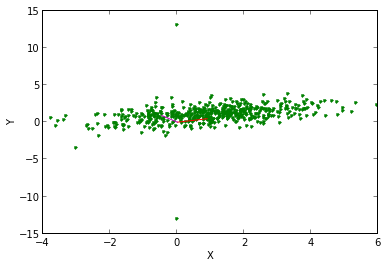
\includegraphics[width=0.7\textwidth]{Exercise_5_files/Exercise_5_fig_00.png}
\par
\end{center}
\end{codeoutput}
\end{codecell}
\subsection{b.) After removing the observation 17, 157:
}
\begin{codecell}
\begin{codeinput}
\begin{lstlisting}
p = data01.shape[1]
data02 = [[0 for i in range(p-2)] for j in range(2)]
r = 0
for j in range(p):
   for i in range(2):
        if (j==16):
            r = 1
            break
        if (j==156):
            r = 2
            break
        data02[i][j-r] = data01[i][j]

fig = plt.figure()
ax = fig.add_subplot(111)
ax.plot(data02[0], data02[1], 'g.')
ax.set_xlabel('X')
ax.set_ylabel('Y')

#plot the two points , which are removed from the dataset
ax.plot(data01[0][16],data01[1][16], 'r.')
ax.plot(data01[0][156],data01[1][156], 'r.')

evals ,evecs = get_PC(data02, 2, 2)

print 'eigenvectors\n', evecs
print 'eigenvalues\n',evals

ax.plot([0, evecs[0,0]],[0,evecs[1,0]],'r-')
ax.plot([0, evecs[0,1]],[0,evecs[1,1]],'m-')
plt.show()
\end{lstlisting}
\end{codeinput}
\begin{codeoutput}
\begin{verbatim}
eigenvectors
[[ 0.93549122 -0.35334993]
 [ 0.35334993  0.93549122]]
eigenvalues
[ 3.04753257  0.63885724]
\end{verbatim}
\begin{center}
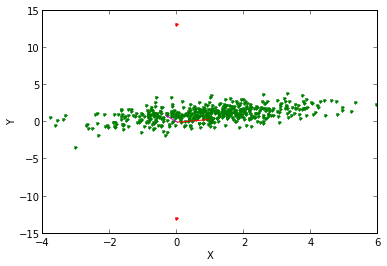
\includegraphics[width=0.7\textwidth]{Exercise_5_files/Exercise_5_fig_01.png}
\par
\end{center}
\end{codeoutput}
\end{codecell}
As we can see from the results, after removing the two noisy points, the eigenvectors changed a lot.
\section{5.2. Whitening}
\subsection{a.) Load the dataset pca4.csv}
\begin{codecell}
\begin{codeinput}
\begin{lstlisting}
data04 = loadtxt('PCAdata2/pca4.csv', delimiter = ',', unpack =True, usecols = (0, 1, 2 ,3), skiprows = 1 )
\end{lstlisting}
\end{codeinput}
\end{codecell}
To check outliers in individual variables:
\begin{codecell}
\begin{codeinput}
\begin{lstlisting}
X = [ i+1 for i in range (len(data04[0,:]))]

for m in range (4):
    fig = plt.figure(m+1)
    ax = fig.add_subplot(111)
    ax.plot(X, data04[m], 'g.')
    ax.set_xlabel('X')
    ax.set_ylabel('Y')
    tmp = "Dimension:",m+1
    plt.title(tmp)
    plt.show()
\end{lstlisting}
\end{codeinput}
\begin{codeoutput}
\begin{center}
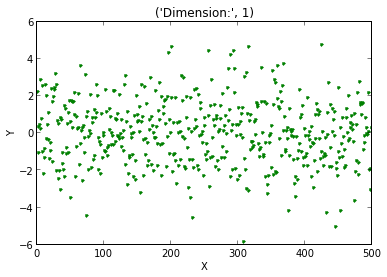
\includegraphics[width=0.7\textwidth]{Exercise_5_files/Exercise_5_fig_02.png}
\par
\end{center}
\begin{center}
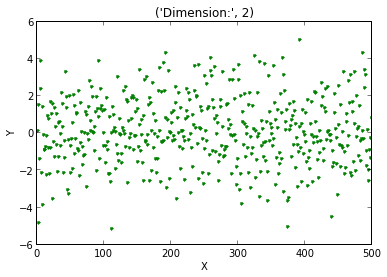
\includegraphics[width=0.7\textwidth]{Exercise_5_files/Exercise_5_fig_03.png}
\par
\end{center}
\begin{center}
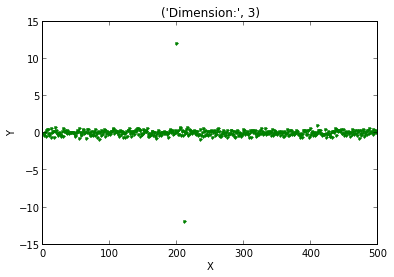
\includegraphics[width=0.7\textwidth]{Exercise_5_files/Exercise_5_fig_04.png}
\par
\end{center}
\begin{center}
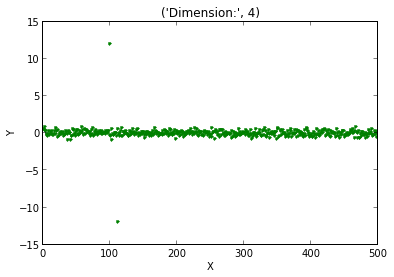
\includegraphics[width=0.7\textwidth]{Exercise_5_files/Exercise_5_fig_05.png}
\par
\end{center}
\end{codeoutput}
\end{codecell}
\subsection{b.) PCA and Scree plot}
\begin{codecell}
\begin{codeinput}
\begin{lstlisting}
evals, evecs = get_PC(data04, 4, 4)
print 'eigenvectors\n', evecs
print 'eigenvalues\n',evals
X = [ 0 for i in range (4)]
Y = [ 0 for i in range (4)]
for i in range(4):
    X[i] = i+1
    Y[i] = evals[i]

fig = plt.figure()
ax = fig.add_subplot(111)
ax.plot(X, Y, 'ro')
ax.plot(X, Y, 'g-')
ax.set_xlabel('X')
ax.set_ylabel('Y')
plt.title('Scree Plot')
plt.show()
\end{lstlisting}
\end{codeinput}
\begin{codeoutput}
\begin{verbatim}
eigenvectors
[[-0.66808317 -0.7440606   0.00612014  0.00111974]
 [-0.74406218  0.66802535 -0.00553581 -0.00910804]
 [ 0.00594509 -0.0054947   0.16150367 -0.98683891]
 [ 0.00100359 -0.00926113 -0.98683761 -0.16144585]]
eigenvalues
[ 4.12502515  1.920516    0.67626699  0.66686614]
\end{verbatim}
\begin{center}
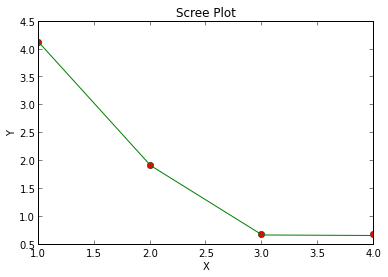
\includegraphics[width=0.7\textwidth]{Exercise_5_files/Exercise_5_fig_06.png}
\par
\end{center}
\end{codeoutput}
\end{codecell}
According to the scree plot, the first two PCs can represent the data well.
\subsection{c.) Whiten the Data}
\begin{codecell}
\begin{codeinput}
\begin{lstlisting}
data_centered = get_CenteredData(data04,4)
evals, evecs = get_PC(data04, 4, 4)
E = matrix(evecs)
Dd = matrix(np.diag([ 1/math.sqrt(evals[i]) for i in range(4)]))
X = matrix(data_centered).T

Z =( X * E) * Dd

data_whiten = [[Z[j,i] for j in range(len(data_centered[0][:]))] for i in range(4)]

print 'data whitened done!'
\end{lstlisting}
\end{codeinput}
\begin{codeoutput}
\begin{verbatim}
data whitened done!
\end{verbatim}
\end{codeoutput}
\end{codecell}
\subsection{d.) Heat plots}
1. covariance matrix of the origin data
\begin{codecell}
\begin{codeinput}
\begin{lstlisting}
C = get_CoMatrix(data04,4)

print matrix(C)

plt.title('1. covariance matrix of the origin data ')
plt.imshow(C,interpolation="nearest",extent=[1,4,4,1])
plt.colorbar()
plt.show()
\end{lstlisting}
\end{codeinput}
\begin{codeoutput}
\begin{verbatim}
[[  2.90437328e+00   1.09555553e+00  -8.51729760e-03   6.28739894e-03]
 [  1.09555553e+00   3.14313145e+00  -2.00219487e-02  -1.08781497e-02]
 [ -8.51729760e-03  -2.00219487e-02   6.67233603e-01  -1.33954775e-03]
 [  6.28739894e-03  -1.08781497e-02  -1.33954775e-03   6.76240053e-01]]
\end{verbatim}
\begin{center}
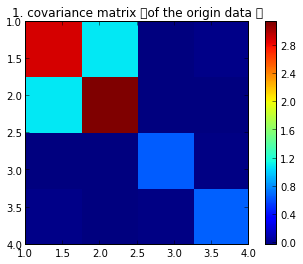
\includegraphics[width=0.7\textwidth]{Exercise_5_files/Exercise_5_fig_07.png}
\par
\end{center}
\end{codeoutput}
\end{codecell}
2. the covariance matrix of the data projected onto PC1-PC4
\begin{codecell}
\begin{codeinput}
\begin{lstlisting}
evals, evecs = get_PC(data04, 4, 4)
B = matrix(evecs)
A = matrix(data04).T
X = A * B
data_projected = [[ X[i,j] for i in range(len(data04[0][:]))] for j in range(4)]

C = get_CoMatrix(data_projected, 4)
print matrix(C)
plt.title('2. the covariance matrix of projected data ')
plt.imshow(C,interpolation="nearest",extent=[1,4,4,1])
plt.colorbar()
plt.show()
\end{lstlisting}
\end{codeinput}
\begin{codeoutput}
\begin{verbatim}
[[  4.12591986e+00  -3.26366538e-15   1.37693676e-17   6.74102701e-17]
 [ -3.26366538e-15   1.92186560e+00  -1.46367293e-18   2.33103467e-18]
 [  1.37693676e-17  -1.46367293e-18   6.76341742e-01  -8.57269171e-15]
 [  6.74102701e-17   2.33103467e-18  -8.57269171e-15   6.66851179e-01]]
\end{verbatim}
\begin{center}
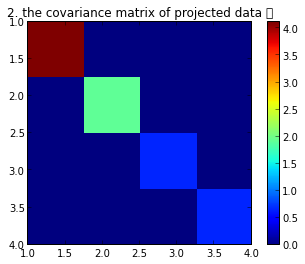
\includegraphics[width=0.7\textwidth]{Exercise_5_files/Exercise_5_fig_08.png}
\par
\end{center}
\end{codeoutput}
\end{codecell}
3. the covariance matrix of the whitened variables
\begin{codecell}
\begin{codeinput}
\begin{lstlisting}
C = get_CoMatrix(data_whiten,4)
print matrix(C)
plt.title('3. the covariance matrix of the whitened variables ')
plt.imshow(C,interpolation="nearest",extent=[1,4,4,1])
plt.colorbar()
plt.show()
\end{lstlisting}
\end{codeinput}
\begin{codeoutput}
\begin{verbatim}
[[  1.00000000e+00  -1.17606120e-15   1.04083409e-17   2.57023678e-17]
 [ -1.17606120e-15   1.00000000e+00  -9.10729825e-18  -1.25902977e-17]
 [  1.04083409e-17  -9.10729825e-18   1.00000000e+00  -1.27597179e-14]
 [  2.57023678e-17  -1.25902977e-17  -1.27597179e-14   1.00000000e+00]]
\end{verbatim}
\begin{center}
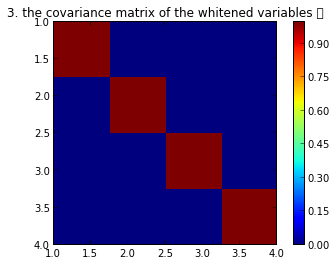
\includegraphics[width=0.7\textwidth]{Exercise_5_files/Exercise_5_fig_09.png}
\par
\end{center}
\end{codeoutput}
\end{codecell}
\section{5.3 Rotation}
\subsection{a.) Dataset Loading and Variables Estimating}
\begin{codecell}
\begin{codeinput}
\begin{lstlisting}
data2b = loadtxt('PCAdata2/pca2b.csv', delimiter = ',', unpack =True, usecols = (0, 1), skiprows = 1 )

fig = plt.figure(1)
ax = fig.add_subplot(111)
ax.set_xlabel('X')
ax.set_ylabel('Y')
ax.set_title('scatter plot of PCAdata2')
ax.plot(data2b[0], data2b[1], 'g.')
fig.show()

plt.clf()
plt.hist(data2b[0], bins=50, color='blue')
plt.title('Histogram of Variable X')
plt.show()

plt.clf()
plt.hist(data2b[1], bins=50, color='blue')
plt.title('Histogram of Variable Y')
plt.show()

#2 vars
heatmap, xedges, yedges = np.histogram2d(data2b[0], data2b[1], bins=20)
extent = [xedges[0], xedges[-1], yedges[0], yedges[-1]]

plt.clf()
plt.title('Histogram of Vars x and y of origin data')
plt.imshow(heatmap,interpolation="nearest", extent=extent)
plt.colorbar()
plt.show()

\end{lstlisting}
\end{codeinput}
\begin{codeoutput}
\begin{center}
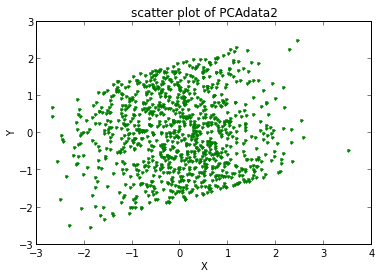
\includegraphics[width=0.7\textwidth]{Exercise_5_files/Exercise_5_fig_10.png}
\par
\end{center}
\begin{center}
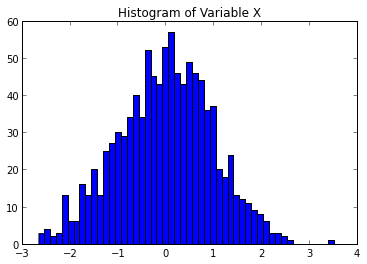
\includegraphics[width=0.7\textwidth]{Exercise_5_files/Exercise_5_fig_11.png}
\par
\end{center}
\begin{center}
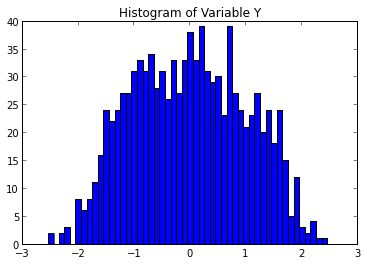
\includegraphics[width=0.7\textwidth]{Exercise_5_files/Exercise_5_fig_12.png}
\par
\end{center}
\begin{center}
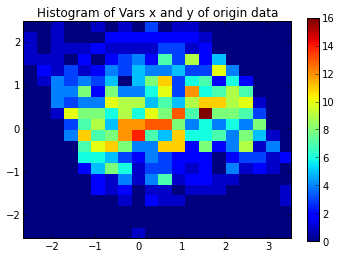
\includegraphics[width=0.7\textwidth]{Exercise_5_files/Exercise_5_fig_13.png}
\par
\end{center}
\end{codeoutput}
\end{codecell}
\subsection{b.) PCA and Projection}
\begin{codecell}
\begin{codeinput}
\begin{lstlisting}
evals, evecs = get_PC(data2b, 2, 2)
print 'eigenvectors\n', evecs
print 'eigenvalues\n',evals
B = matrix(evecs)
A = matrix(data2b).T
X = A * B
data2b_projected = [[ X[i,j] for i in range(len(data02[0][:]))] for j in range(2)]

fig = plt.figure()
ax = fig.add_subplot(111)
ax.set_title('scatter plot of projected data in PC coordinate System')
ax.set_xlabel('X')
ax.set_ylabel('Y')
ax.plot(data2b_projected[0], data2b_projected[1], 'g.')
plt.show()


\end{lstlisting}
\end{codeinput}
\begin{codeoutput}
\begin{verbatim}
eigenvectors
[[-0.90630779 -0.42261826]
 [ 0.42261826 -0.90630779]]
eigenvalues
[ 0.94875444  1.04924556]
\end{verbatim}
\begin{center}
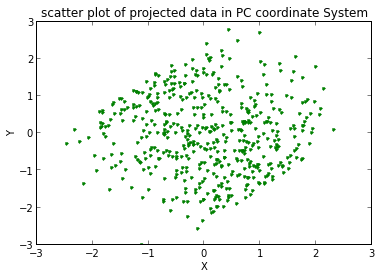
\includegraphics[width=0.7\textwidth]{Exercise_5_files/Exercise_5_fig_14.png}
\par
\end{center}
\end{codeoutput}
\end{codecell}
\subsection{c.) Whiten the data and do rotation of 45 degree}
\begin{codecell}
\begin{codeinput}
\begin{lstlisting}
data2b_centered = get_CenteredData(data2b,2)
evals, evecs = get_PC(data2b, 2, 2)
E = evecs
D = evals


data2b_whiten = [[0 for j in range(len(data2b_centered[0][:]))] for i in range(2)]


for j in range(len(data2b_centered[0][:])):
    for i in range(2):
        data2b_whiten[i][j] = 0
        for m in range(2):
            data2b_whiten[i][j] = data2b_centered[m][j] * E[m,i]  + data2b_whiten[i][j]
        data2b_whiten[i][j] = 1/math.sqrt(evals[i]) * data2b_whiten[i][j]

print 'data whitened done!'


R = matrix ([[math.cos(45), -math.sin(45)],[math.sin(45),math.cos(45)]])
Z = matrix(data2b_whiten).T
Zrot = (R * Z.T).T
data2b_rotate = [[Zrot[j,i] for j in range(len(data2b_centered[0][:]))] for i in range(2)]


print 'After Rotation..'
fig = plt.figure()
ax = fig.add_subplot(111)
ax.set_title('scatter plot of rotated data')
ax.set_xlabel('X')
ax.set_ylabel('Y')
ax.plot(data2b_rotate[0], data2b_rotate[1], 'g.')
plt.show()

\end{lstlisting}
\end{codeinput}
\begin{codeoutput}
\begin{verbatim}
data whitened done!
After Rotation..
\end{verbatim}
\begin{center}
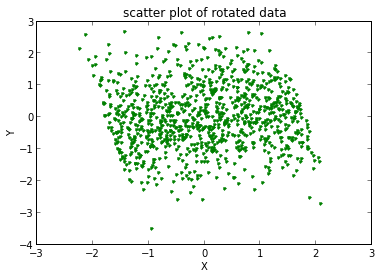
\includegraphics[width=0.7\textwidth]{Exercise_5_files/Exercise_5_fig_15.png}
\par
\end{center}
\end{codeoutput}
\end{codecell}
\subsection{d. marginal densities of variables}
whitened variables zi
\begin{codecell}
\begin{codeinput}
\begin{lstlisting}
plt.clf()
plt.hist(Z[:,0], bins=50, color='blue')
plt.title('Variable X of whitened data')
plt.show()

plt.clf()
plt.hist(Z[:,1], bins=50, color='blue')
plt.title('Variable Y of whitend data')
plt.show()

#2 vars
heatmap, xedges, yedges = np.histogram2d(data2b_whiten[0], data2b_whiten[1], bins=20)
extent = [xedges[0], xedges[-1], yedges[0], yedges[-1]]

plt.clf()
plt.title('x and y of whitend data')
plt.imshow(heatmap,interpolation="nearest", extent=extent)
plt.colorbar()
plt.show()
\end{lstlisting}
\end{codeinput}
\begin{codeoutput}
\begin{center}
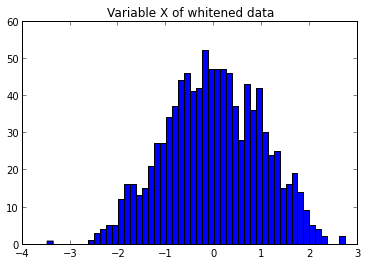
\includegraphics[width=0.7\textwidth]{Exercise_5_files/Exercise_5_fig_16.png}
\par
\end{center}
\begin{center}
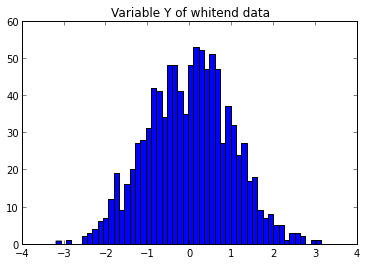
\includegraphics[width=0.7\textwidth]{Exercise_5_files/Exercise_5_fig_17.png}
\par
\end{center}
\begin{center}
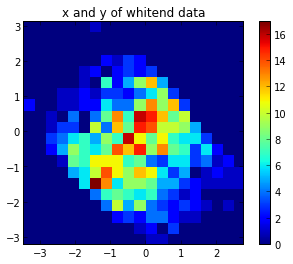
\includegraphics[width=0.7\textwidth]{Exercise_5_files/Exercise_5_fig_18.png}
\par
\end{center}
\end{codeoutput}
\end{codecell}
the rotated variables Zrot

\begin{codecell}
\begin{codeinput}
\begin{lstlisting}
plt.clf()
plt.hist(Zrot[:,0], bins=50, color='blue')
plt.title('Variable X of rotated data')
plt.show()

plt.clf()
plt.hist(Zrot[:,1], bins=50, color='blue')
plt.title('Variable Y of rotated data')
plt.show()

#2 vars
heatmap, xedges, yedges = np.histogram2d(data2b_rotate[0], data2b_rotate[1], bins=20)
extent = [xedges[0], xedges[-1], yedges[0], yedges[-1]]
plt.clf()
plt.title('X and Y of rorated data')
plt.imshow(heatmap,interpolation="nearest", extent=extent)
plt.colorbar()
plt.show()
\end{lstlisting}
\end{codeinput}
\begin{codeoutput}
\begin{center}
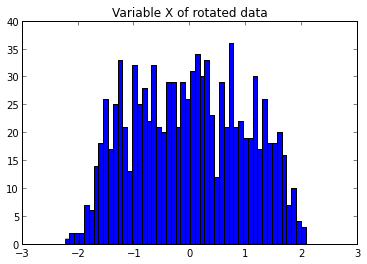
\includegraphics[width=0.7\textwidth]{Exercise_5_files/Exercise_5_fig_19.png}
\par
\end{center}
\begin{center}
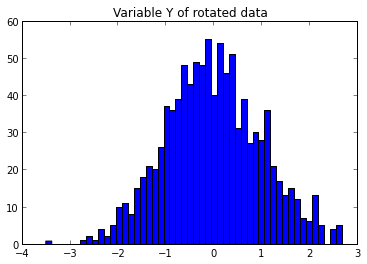
\includegraphics[width=0.7\textwidth]{Exercise_5_files/Exercise_5_fig_20.png}
\par
\end{center}
\begin{center}
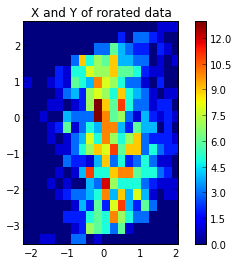
\includegraphics[width=0.7\textwidth]{Exercise_5_files/Exercise_5_fig_21.png}
\par
\end{center}
\end{codeoutput}
\end{codecell}
\section{Comparation of Covariance Matrix}
\begin{codecell}
\begin{codeinput}
\begin{lstlisting}
C1 = get_CoMatrix(data2b,2)
print matrix(C1)
plt.title('origin data ')
plt.imshow(C1,interpolation="nearest",extent=[1,2,2,1])
plt.colorbar()
plt.show()
\end{lstlisting}
\end{codeinput}
\begin{codeoutput}
\begin{verbatim}
[[ 0.96670278  0.03849033]
 [ 0.03849033  1.03129722]]
\end{verbatim}
\begin{center}
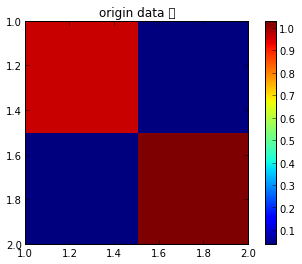
\includegraphics[width=0.7\textwidth]{Exercise_5_files/Exercise_5_fig_22.png}
\par
\end{center}
\end{codeoutput}
\end{codecell}
\begin{codecell}
\begin{codeinput}
\begin{lstlisting}
C2 = get_CoMatrix(data2b_whiten,2)
print matrix(C2)
plt.title('whitened data ')
plt.imshow(C2,interpolation="nearest",extent=[1,2,2,1])
plt.colorbar()
plt.show()
\end{lstlisting}
\end{codeinput}
\begin{codeoutput}
\begin{verbatim}
[[  1.00000000e+00  -2.29661125e-16]
 [ -2.29661125e-16   1.00000000e+00]]
\end{verbatim}
\begin{center}
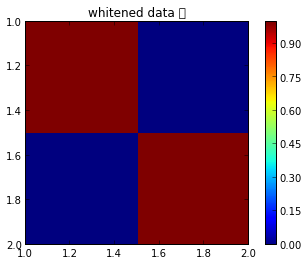
\includegraphics[width=0.7\textwidth]{Exercise_5_files/Exercise_5_fig_23.png}
\par
\end{center}
\end{codeoutput}
\end{codecell}
\begin{codecell}
\begin{codeinput}
\begin{lstlisting}
C3 = get_CoMatrix(data2b_rotate,2)
print matrix(C3)
plt.title('rotated data ')
plt.imshow(C3,interpolation="nearest",extent=[1,2,2,1])
plt.colorbar()
plt.show()
\end{lstlisting}
\end{codeinput}
\begin{codeoutput}
\begin{verbatim}
[[  1.00000000e+00  -1.77809156e-17]
 [ -1.77809156e-17   1.00000000e+00]]
\end{verbatim}
\begin{center}
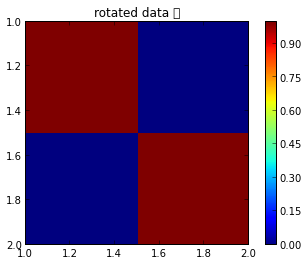
\includegraphics[width=0.7\textwidth]{Exercise_5_files/Exercise_5_fig_24.png}
\par
\end{center}
\end{codeoutput}
\end{codecell}
As we can see, the whitened dataset is uncorrelated, even if it is rotated.
\end{document}
